\documentclass[logo,reportComp]{thesis}
\usepackage[python,pseudo,linenum]{mypackage}
\hypersetup{colorlinks=false,urlbordercolor=red}
\usepackage{relsize}
\usepackage{subcaption}
% \usepackage{underscore}
\usepackage[nottoc]{tocbibind}

\lstset{texcl=true,escapechar=\#\\\_}

\setcounter{secnumdepth}{4}
\titleformat{\paragraph}{\bfseries}{\alph{paragraph})~~}{0em}{}
\titlespacing*{\paragraph}{0pt}{0pt}{0pt}[0pt]

\title{人工神经网络}
\subtitle{Lab 4:卷积神经网络(CNN)}
\school{数据科学与计算机学院}
\author{陈鸿峥}
\classname{17大数据与人工智能}
\stunum{17341015}
\headercontext{人工神经网络作业}

\let\emph\relax % there's no \RedeclareTextFontCommand
\DeclareTextFontCommand{\emph}{\kaiti\em}
\AtBeginEnvironment{quote}{\kaiti\small}

\begin{document}

\maketitle
\tableofcontents

\newpage

\section{均方差损失}
均方差\verb'MSELoss'的实现在\verb'01.toy.py'中,核心代码如下。

\lstinputlisting[linerange={60-60,68-71}]{../code/01.toy.py}

注意输入的\verb'input'是每个类别的概率值,而\verb'target'仅仅是一个目标类别。
故需要先将\verb'target'用独热码编码为与\verb'input'维度一致,这里用到NumPy的fancy indexing进行独热码的创建。

运行结果如图\ref{fig:t1}所示,可见成功学习到异或规律。
\begin{figure}[H]
\centering
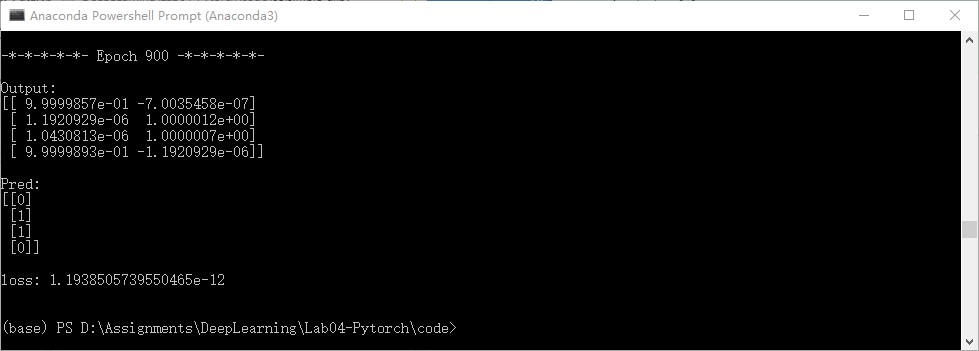
\includegraphics[width=\linewidth]{fig/T1.jpg}
\caption{题1结果}
\label{fig:t1}
\end{figure}

\section{学习数数}
CNN的模型在\verb'02.learn-to-count.py'中,核心代码如下。

\lstinputlisting[linerange={30-30,38-50}]{../code/02.learn-to-count.py}

运行结果如图\ref{fig:t2}所示,可见在MNIST数据集上分类准确率达到了98.04\%。
\begin{figure}[H]
\centering
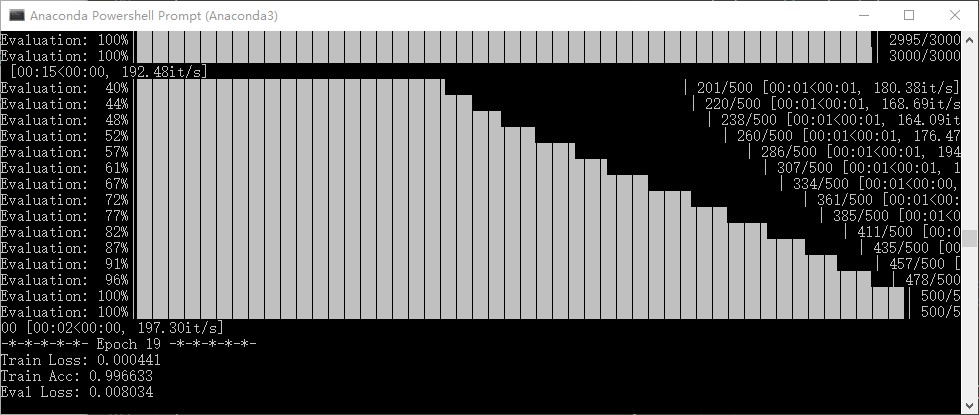
\includegraphics[width=\linewidth]{fig/T2.jpg}
\caption{题2结果}
\label{fig:t2}
\end{figure}

\section{简单可用的AI}
在本实验中我实现了两个网络LeNet5\cite{lenet}和VGG16\cite{vgg},网络定义参见\verb'mynet.py',完整训练代码见\verb'03.simple-ai.py'。
为了避免过拟合,我采取了以下措施:
\begin{itemize}
    \item \textbf{Dropout}:在全连接层前面添加\verb'nn.Dropout',以一定概率(默认为$0.5$)隐藏神经元
    \item \textbf{批归一化}:在每个卷积层后面添加\verb'nn.BatchNorm2D',实现批归一化(batch normalization)
    \item \textbf{早停}:在\verb'myutils.py'中实现了\verb'EarlyStopping'类,通过判断验证集上的损失是否持续下降,来决定是否继续训练。
\end{itemize}

LeNet和VGG的代码如下,都用\verb'nn.Sequential'进行封装,由于论文中对其网络架构已经描述得很清楚了,故在PyTorch上只需将各层合并起来即可。
这里提前将论文中提及的不同层数的网络结构用\verb'vgg_config'进行描述,在网络初始化过程中才将对应的卷积层插入。
\lstinputlisting{../code/mynet.py}

早停的代码实施如下,其中\verb'patience'即可忍耐的损失不下降的轮数。
\lstinputlisting{../code/myutils.py}

训练和验证的部分复用了\verb'02.learn-to-count.py'的代码。
同时增添了对训练、测试损失及精度的存储(以\verb'.npz'格式),方便后续的可视化工作。
另外由于网络训练实在太慢,故在本实验中我只选择了LeNet5和VGG16进行训练,同时使用了GPU\footnote{Nvidia GTX 1050, CUDA 10.1}进行加速,批次大小$32$,学习率为$10^{-3}$,采用Adam优化器。

最终实验结果如下,图\ref{fig:loss}为损失函数变化,图\ref{fig:acc}为精度变化。
可以看到采取了早停策略,LeNet5才不会继续过拟合,其在测试集的最高准确率为64.56\%。
对于VGG16,同样采取了早停策略\footnote{当然最好是将patience设大一些,同时达到patience后降低学习率,不过为了方便本实验并没有做学习率衰减的测试。},可以看到对于最后几个epoch,损失函数和精度的变化都已经变缓了,因此早停可以有效避免继续训练的过拟合。
\begin{figure}[H]
\begin{subfigure}{0.5\textwidth}
\centering
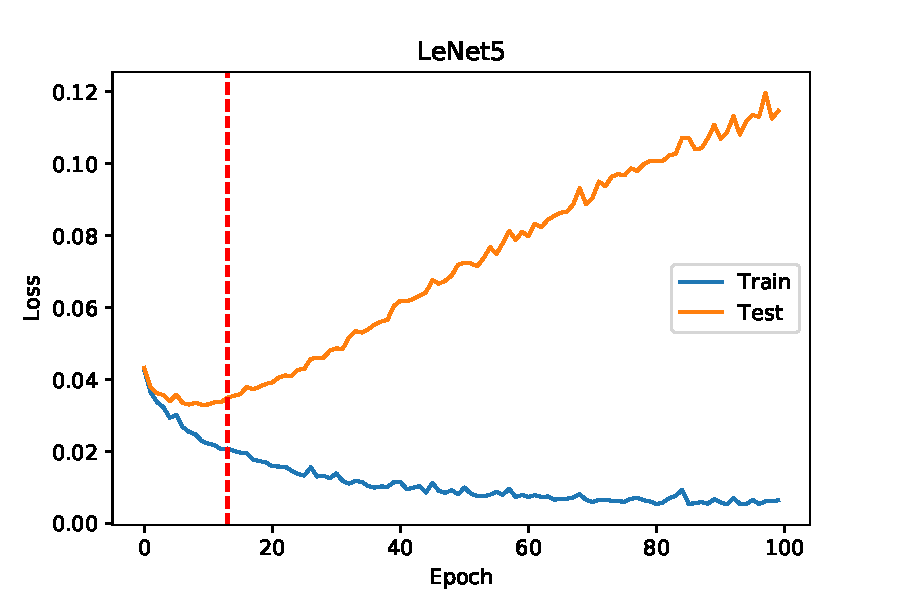
\includegraphics[width=\linewidth]{fig/LeNet5_loss.pdf}
\caption{LeNet5损失(红线为早停点)}
\end{subfigure}
\begin{subfigure}{0.5\textwidth}
\centering
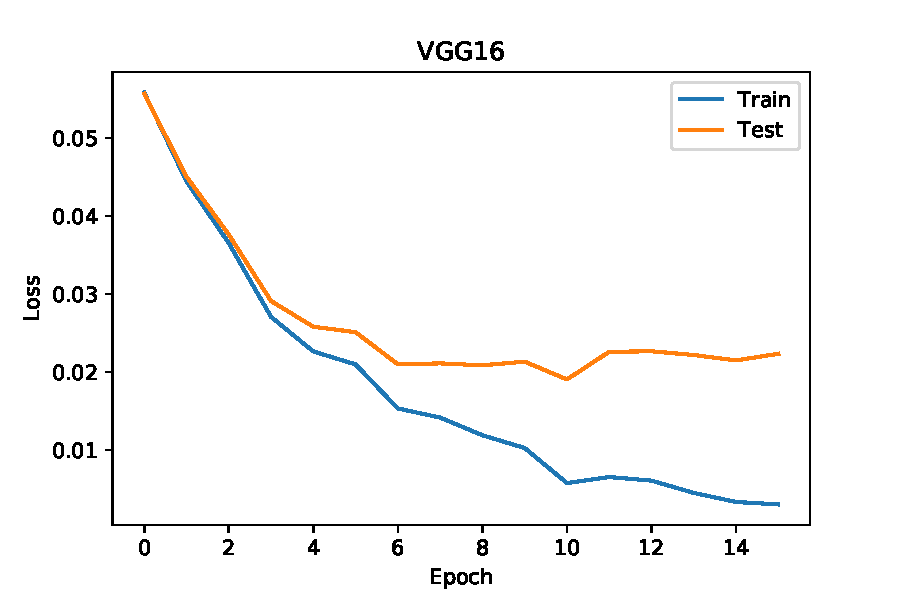
\includegraphics[width=\linewidth]{fig/VGG16_loss.pdf}
\caption{VGG16损失}
\end{subfigure}
\caption{训练集及测试集Loss变化}
\label{fig:loss}
\end{figure}

\begin{figure}[H]
\begin{subfigure}{0.5\textwidth}
\centering
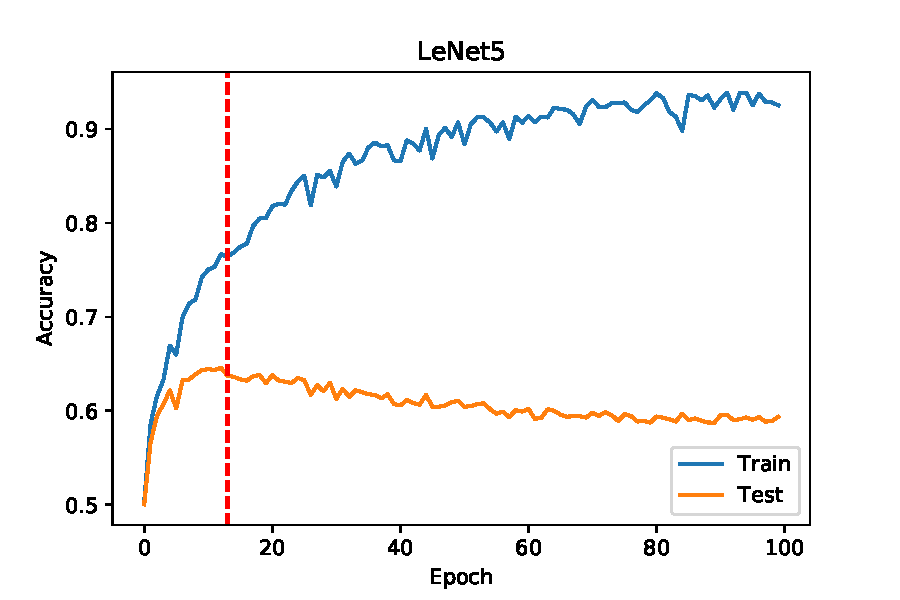
\includegraphics[width=\linewidth]{fig/LeNet5_acc.pdf}
\caption{LeNet5准确率(红线为早停点)}
\end{subfigure}
\begin{subfigure}{0.5\textwidth}
\centering
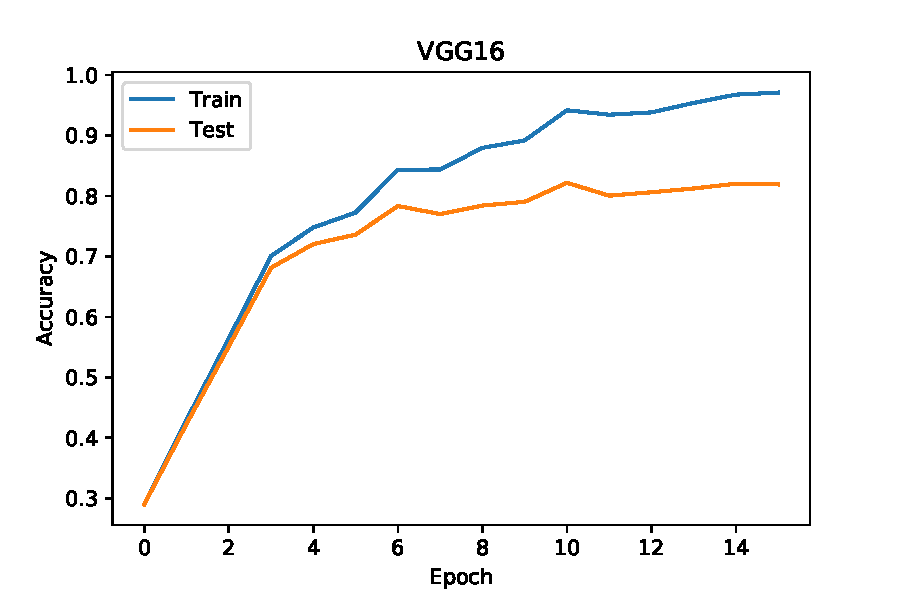
\includegraphics[width=\linewidth]{fig/VGG16_acc.pdf}
\caption{VGG16准确率}
\end{subfigure}
\caption{训练集及测试集准确率变化}
\label{fig:acc}
\end{figure}

图\ref{fig:comparison}展示了两个网络的准确率比较,它们都超过了60\%的基准值,同时VGG16明显好于LeNet5的性能,最高达到了82.18\%的准确率。
不过由于时间和硬件的限制,本实验并没有继续做更多的调优,理论上VGG的准确率可以达到更高。
\begin{figure}[H]
\centering
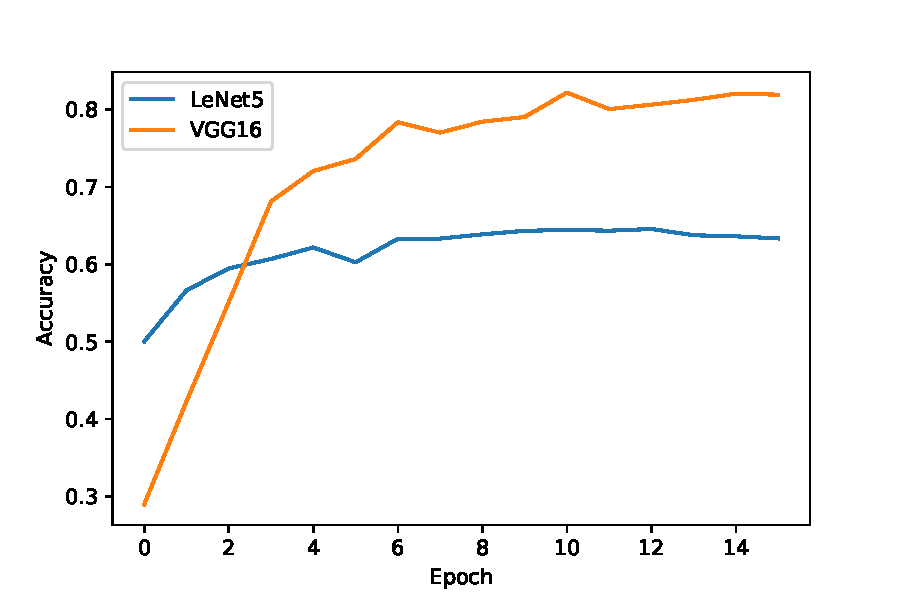
\includegraphics[width=0.6\linewidth]{fig/acc_comparison.pdf}
\caption{LeNet5与VGG16在CIFAR-10测试集上准确率比较}
\label{fig:comparison}
\end{figure}

\begin{thebibliography}{99}
\bibitem{lenet} Yann Lecun, Léon Bottou Bottou, Yoshua Bengio, and Patrick Haffner, "Gradient-based learning applied to document recognition," in Proceedings of the IEEE, vol. 86, no. 11, pp. 2278-2324, Nov. 1998.
\bibitem{vgg} Karen Simonyan, and Andrew Zisserman, "Very Deep Convolutional Networks for Large-Scale Image Recognition," in Proceedings of the International Conference of Learning and Representation (ICLR), 2015.
\end{thebibliography}

\end{document}